\documentclass[11pt, oneside]{article}   	% use "amsart" instead of "article" for AMSLaTeX format
\usepackage[margin=0.75in]{geometry}                		% See geometry.pdf to learn the layout options. There are lots.
\usepackage[utf8]{inputenc}
\geometry{letterpaper}                   		% ... or a4paper or a5paper or ... 
%\geometry{landscape}                		% Activate for rotated page geometry
%\usepackage[parfill]{parskip}    		% Activate to begin paragraphs with an empty line rather than an indent
\usepackage{graphicx}				% Use pdf, png, jpg, or eps§ with pdflatex; use eps in DVI mode
\usepackage{wrapfig}
								% TeX will automatically convert eps --> pdf in pdflatex		
\usepackage{amssymb}
\usepackage{amsmath}
\usepackage{mathtools}

\usepackage{xcolor}
\usepackage{framed}

\usepackage{listings}
%usage: \lstinputlisting[language=Python]{script.py}


\definecolor{shadecolor}{RGB}{0,113,186}
\usepackage{xparse}
\NewDocumentCommand{\DIV}{om}{%
  \IfValueT{#1}{\setcounter{#2}{\numexpr#1-1\relax}}%
  \csname #2\endcsname
}

\definecolor{codegreen}{rgb}{0,0.6,0}
\definecolor{codegray}{rgb}{0.5,0.5,0.5}
\definecolor{codepurple}{rgb}{0.58,0,0.82}
\definecolor{backcolour}{rgb}{0.95,0.95,0.92}
\usepackage{xcolor}

\title{Project Euler, Problem 144:\\\large{Investigating Multiple Reflections of a Laser Beam}}
\author{John Butler}
\date{}							% Activate to display a given date or no date

\newcommand{\code}[1]{\colorbox{backcolour}{\texttt{#1}}}

\lstdefinestyle{mystyle}{
    backgroundcolor=\color{backcolour},   
    commentstyle=\color{codegreen},
    keywordstyle=\color{magenta},
    numberstyle=\tiny\color{codegray},
    stringstyle=\color{codepurple},
    basicstyle=\ttfamily\footnotesize,
    breakatwhitespace=false,         
    breaklines=true,                 
    captionpos=b,                    
    keepspaces=true,                 
    numbers=left,                    
    numbersep=5pt,                  
    showspaces=false,                
    showstringspaces=false,
    showtabs=false,                  
    tabsize=4
}

\lstset{style=mystyle}
\begin{document}
\maketitle

\tableofcontents
\newpage

\section{Problem Description}
	Consider an ellipse with the equation $4x^2+y^2 = 100$ with the section $x\in [-0.01, 0.01]$ missing from the
	top. A straight lightbeam is shined in at $(0,10.1)$ and hits the ellipse at $(1.4, -9.6)$. The light then
	reflects off the inside until it exits through the 0.02 wide opening it entered from.\\
	It's given that the slope of the tangent of the ellipse at any point is $\frac{-4x}{y}$ and that
	the angle of incidence equals the angle of reflection, that is the angle between the incoming beam and the
	tangent line equals the angle between the outgoing beam and the tangent.
	
\section{Theorems whose results aid in my solution}

\subsection{The ellipse $4x^2 + y^2 = 100$ can be rewritten as $y = \pm \sqrt{100 - 4x^2}$}
	\begin{align*}
		4x^2 + y^2 &= 100\\
		y^2 &= 100 - 4x^2\\
		y &= \pm \sqrt{100 - 4x^2}
	\end{align*}

\subsection{Given some line, $y=mx+b$ that intersects the ellipse $4x^2+y^2=100$, then the x coordinates of the 
intersection points are at $$x_{+,-} = \frac{-2bm \pm \sqrt{(2bm)^2 - 4(4+m^2)(b^2 - 100)}}{2(4 + m^2)}$$ 
meaning the points lie at $(x_+,mx_++b)$ and $(x_-, mx_- + b)$}
	\begin{align*}
		4x^2 + y^2 = 100 &\iff y = \pm \sqrt{100-4x^2 }\\
		\text{The intersections happens when the line}&\text{ and ellipse have the same $x$ and $y$ coordinates.}\\
		\therefore mx+b = y &= \pm \sqrt{100 - 4x^2}\\
		mx+b  &= \pm \sqrt{100 - 4x^2}\\
		(mx+b)^2 &= (\pm\sqrt{100 - 4x^2})^2\\
		m^2x^2 + 2bmx + b^2 &= 100 - 4x^2\\
		(m^2 + 4)x^2 + (2bm)x + (b^2 - 100) &= 0\\
		\text{We can solve for }&x\text{ using the quadradic formula}\\
		x_{+,-} &= \frac{-2bm \pm \sqrt{(2bm)^2 - 4(4+m^2)(b^2 - 100)}}{2(4 + m^2)}\\
		\text{Truthfully, this can be simpli}&\text{fied, but I believe this is simpler to compute.}\\
		\text{The intersection point must be}&\text{ on the line, so if we plug in each $x$, we get:}\\
		y_+ &= mx_++b\\
		\text{and }y_- &= mx_- + b\\
		\text{So the intersection points are }&(x_+,mx_++b) \text{ and }(x_-, mx_- + b)
	\end{align*}

\newpage
\subsection{Lemma: if $m$ is the slope of a line, and $\theta$ is the angle between that line and the x-axis,
then $$\tan\theta = m$$}
	%\begin{wrapfigure}{r}{0.25\textwidth}
	%	\centering
	%	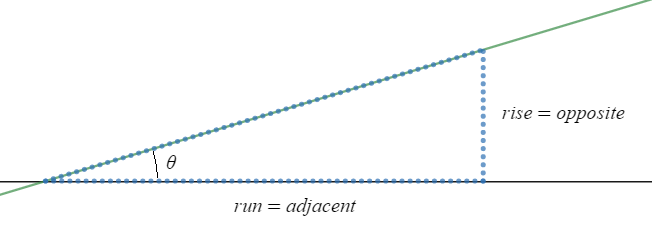
\includegraphics[width=0.5]{2.3 visual aid clean.png}
	%\end{wrapfigure}
	Consider the figure below. I started by taking an arbitrary line, then I drew a vertical line from which 
	I constructed a right triangle. To calculate the slope of the line, I divided the "rise" and the "run"
	of the line over this triangle. The rise measures the change in the y-coordinate, and since the opposite
	edge of the triangle is exactly vertical, the length of that line is the rise. Similarly, the bottom edge
	of the triangle is exactly horizontal, so its length is the run. The slope is the ratio of those to edges.
	Now let's consider what the tangent of the angle between the line and the x-axis is. Well it's the ratio of
	the lengths of the opposite edge to the adjacent edge to the angle. This two perform exactly the same 
	operation, thus they are equal.
	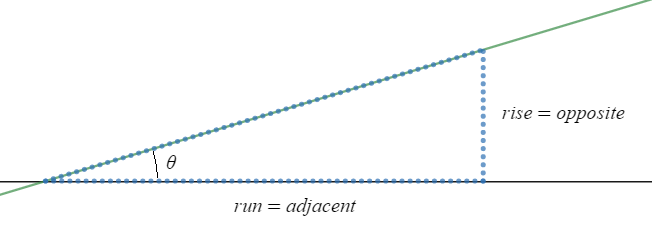
\includegraphics{2.3 visual aid clean.png}

\subsection{If $m_i, m_r, m_t$ are the slopes of the incoming line, reflected line, 
and tangent line, respectively, then $$m_r = \tan\left(2\times \arctan(m_t) - \arctan(m_i)\right)$$}
	\begin{wrapfigure}{r}{0.5\textwidth}
		\centering
		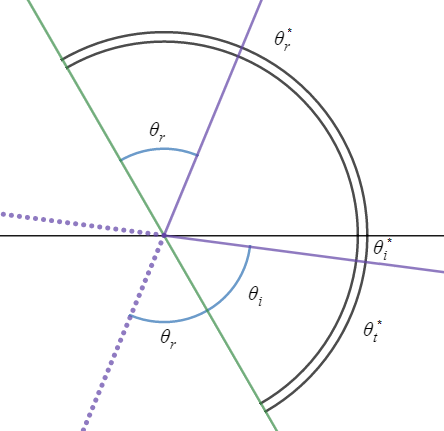
\includegraphics[width=0.5\textwidth]{2.4 visual aid.png}
	\end{wrapfigure}
	Consider $\theta_i$ and $\theta_r$, the angle of incidence and the angle of reflection.  These angles are 
	defined as the angle between the tangent line and either the line of incidence and reflection. Therefore,
	in an absolute sense, $\theta_i = |\theta_t^*-\theta_i^*|$ and \\$\theta_r = |\theta_t^*-\theta_r^*|$, where
	$\theta^*$ represents the angle between a line and the x-axis. Applying lemma 2.3, we get 
	$\begin{cases}
		\theta_i=|\arctan{m_i} - \arctan{m_t}|\\
		\theta_r=|\arctan{m_r} -\arctan{m_t}|
	\end{cases}$.
	Since both lines are on the same side of the tangent line, one angle will be positive and one will be negative, 
	so we get
	$\begin{cases}
		\theta_i=\arctan{m_i} - \arctan{m_t}\\
		\theta_r=\arctan{m_t} - \arctan{m_r}
	\end{cases}$
	or 
	$\begin{cases}
		\theta_i=\arctan{m_t} - \arctan{m_i}\\
		\theta_r=\arctan{m_r} - \arctan{m_t}
	\end{cases}$.
	If we remember that $\theta_i=\theta_r$, in either case, we get
	\begin{align*}
		(\arctan m_i -\arctan m_t ) &= -(\arctan m_r - \arctan m_t )\\
		\arctan m_i  - \arctan m_t  &= \arctan m_t  -\arctan m_r \\
		\arctan m_r  &= 2\times \arctan m_t  - \arctan m_i \\
		m_r &= \tan\left(2\times \arctan m_t  - \arctan m_i \right)
	\end{align*}\\

\section{Application to Code}
	The core of this problem is being able to find the reflection of arbitrary lines at arbirary points on the 
	ellipse. So how do we do that? Well there's certainly a few ways to go about it, but I'm constructing the 
	reflected line from the point slope form, which makes most sense to me. The point is the intersection point
	that we learned how to calculate from result 2.2, then we find the slope using result 2.4. There is one problem,
	though; there are two intersection points. The solution I had is that I pass both the line and the previous 
	intersection point. Then I compute both points and only use the one that is distinct.
	
	%\lstinputlisting[language=Java]{Outline.java}

\section{Complexity Analysis / Further Optimizations and Considerations}
	%Direction
	%squish ellipse to circle
	%rational, so seemingly would make a star and we could figure it out based on that.


\end{document}  
